 
 %BSP Bild
%\begin{figure}[h]
%\centering
%\includegraphics[width=7cm,height=2.8cm]{Fotos/logo.jpg}
%\end{figure}

%BSP Sektion
%\section{Test}
%\subsection{Umsetzung}
%\subsubsection{Eingabe}

%BSP Aufzählung
%\begin{enumerate}
%\item Wie realisieren wir den Roboter mechanisch?
%\item Wie lässt sich das Einlesen des Sudokus umsetzen?
%\item Wie implementieren wir den Algorithmus?
%\end{enumerate}

%BSP Aufzählung
%\begin{itemize}
%\item Helligkeitssensor
%\item Farbsensor
%\end{itemize}


%-------------------
%Beginn des Kopfbereiches
%-------------------

%Wir verwenden eine DIN-A4-Seite und die Schriftgrš§e 12.
\documentclass[a4paper,13pt]{scrartcl} 

%ein Versuch die Silbentrennung auszuschalten
%\hyphenpenalty=10000
%\exhyphenpenalty=10000
\usepackage[none]{hyphenat} 
\sloppy

%Fuer Abbildungsverzeichnis
\usepackage{graphicx}

%Diese drei Pakete benštigen wir fŸr die Umlaute, Deutsche Silbentrennung etc.
\usepackage[utf8x]{inputenc}
\usepackage[ngerman]{babel}
\usepackage[T1]{fontenc}

%Für Zeilenabstände
\usepackage{setspace}

% Für Bilder 
\usepackage{graphicx}

%sorgt dafür, dass deutsche Anführungszeichen in Zitaten
\usepackage[babel,german=quotes]{csquotes}

%Das Paket erzeugt ein anklickbares Verzeichnis in der PDF-Datei.
\usepackage{hyperref}

\usepackage{titleref}

%für Eurosymbole
\usepackage{eurosym}

\usepackage{enumitem}
%Caption in Minipage
\usepackage{caption}
% Stil der Zitate und der Bibliographie
\bibliographystyle{unsrt}

% Einbindung von Quellcode
\usepackage{listings}  



%Das Paket wird fŸr die anderthalb-zeiligen Zeilenabstand benštigt
\usepackage{setspace}

%Fuer Abbildungsverz im Inhaltsverz
\usepackage{tocbibind}

\usepackage{pdfpages}

\usepackage{amssymb}
\usepackage{amsmath}
\usepackage{amsthm}

%Für Bögen über Strecken
\usepackage{arcs}

% Tims Zeug
\usepackage{contour}
\usepackage{ulem}
\renewcommand{\ULdepth}{1.8pt}
\contourlength{0.8pt}
\newcommand{\myuline}[1]{%
  \uline{\phantom{#1}}%
  \llap{\contour{white}{#1}}%
}


%EinrŸckung eines neuen Absatzes
\setlength{\parindent}{0em}

%Definition der Ränder
\usepackage[paper=a4paper,left=30mm,right=30mm,top=30mm,bottom=30mm]{geometry} 

%Abstand der Fußnoten
%\deffootnote{1em}{1em}{\textsuperscript{\thefootnotemark\ }}

%Regeln, bis zu welcher Tiefe (section,subsection,subsubsection) †berschriften angezeigt werden sollen (Anzeige der †berschriften im Verzeichnis / Anzeige der Nummerierung)
%\setcounter{tocdepth}{3}
%\setcounter{secnumdepth}{3}

% Einbindung von Quellcode

\usepackage{xcolor}
\usepackage{listings}
\lstset{
	numbers=left, 
	numberstyle=\small, 
	numbersep=8pt,
	language=JAVA, 
	frame = single, 
	framexleftmargin=15pt}

\renewcommand{\ttdefault}{pcr}	% Typewriter auf Courier
%Text \texttt{Text} \textbf{Text} \texttt{\textbf{Text}}
%
\definecolor{keywords}{RGB}{255,0,90}
\definecolor{comments}{RGB}{0,0,113}
\definecolor{dunkelrot}{RGB}{160,0,0}
\definecolor{dunkelgruen}{RGB}{0,150,0}
%
\lstset{language=Python
	,frame=single
	,basicstyle=\ttfamily
	,keywordstyle=\color{blue}
	,commentstyle=\color{dunkelgruen}\slshape
	,stringstyle=\color{black}
	,showstringspaces=false
	,identifierstyle=\color{black}
	,emph={False,True,range}
	,emphstyle=\color{black}\bfseries
	,tabsize=2
}
%-------------------
%Ende des Kopfbereiches
%-------------------

%-------------------
%Hier beginnt der Text deiner Hausarbeit
%-------------------
\begin{document}
%Beginn der Titelseite
\begin{titlepage}
\begin{center}
% Upper part of the page
\includegraphics[width=0.5\textwidth]{photos/lmg8.png}\\[1.5cm]    
%\textsc{\LARGE University of Beer}\\[1.5cm]
\textsc{\Large Software-Projekt im Fach Informatik }\\[0.4cm]
\textsc{Leitung: Frau Müller}\\[0.4cm]
% Title
\hrule 
%scheint die Linie zu machen
%es gibt medskip bigskip und smallskip
\bigskip


{ \huge \bfseries Role-Play-Game }\\[0.3cm]
\medskip
\hrule
\bigskip
\medskip


% Author and supervisor
\begin{minipage}{0.4\textwidth}
\begin{flushleft} \large


\end{flushleft}
\end{minipage}
\hfill
\begin{minipage}{0.4\textwidth}
\begin{flushright} \large
\bigskip
\medskip
Jasper Hundsdorfer \\
Joshua Kieburg\\
Tobias Palzer\\
Yannick Müller\\

\end{flushright}
\end{minipage}

\vfill

% Bottom of the page
{\large 21. Oktober 2019} 

\end{center}

\end{titlepage}
%Ende der Titelseite

%Inhaltsverzeichnis (aktualisiert sich erst nach dem zweiten Setzen)
\tableofcontents

\renewcommand*{\listoffigures}{%
	\begingroup
	\tocchapter
	\tocfile{\listfigurename}{lof}
	\endgroup
}

\pagestyle{plain}

\newpage

\section {Lastenheft}
\label{Lastenheft}
    \subsection{UR001}
        \hspace*{10mm} \textbf{Aussage} 
            \begin{addmargin}{20mm} 
                Role-Play-Game soll eine graphische Benutzeroberfläche haben.
            \end{addmargin}
        \hspace*{10mm} \textbf{Priorität A}
    \subsection{UR002}
        \hspace*{10mm} \textbf{Aussage} 
            \begin{addmargin}{20mm} 
                Role-Play-Game soll erstellbare Helden enthalten. Dieser soll in Runden gegen Monster kämpfen.
            \end{addmargin}
        \hspace*{10mm} \textbf{Priorität A}
    \subsection{UR003}
        \hspace*{10mm} \textbf{Aussage} 
            \begin{addmargin}{20mm}
                Eine Animation des Kampfes soll zu sehen sein.
            \end{addmargin}
        \hspace*{10mm} \textbf{Priorität B}
    \subsection{UR004}
        \hspace*{10mm} \textbf{Aussage} 
            \begin{addmargin}{20mm}
                Role-Play-Game soll verschiedene Monster und Helden, bspw. Magier und Krieger enthalten, welche unterschiedlich sich durch ihr Aussehen unterscheiden.
            \end{addmargin}
        \hspace*{10mm} \textbf{Priorität A}
    \subsection{UR005}
        \hspace*{10mm} \textbf{Aussage} 
            \begin{addmargin}{20mm}
                Role-Play-Game soll verschiedene Monster und Helden, bspw. Magier und Krieger enthalten, welche sich auch in Stärken bzw. Fähigkeiten unterscheiden.
            \end{addmargin}
        \hspace*{10mm} \textbf{Priorität B}
    \subsection{UR006}
        \hspace*{10mm} \textbf{Aussage} 
            \begin{addmargin}{20mm}
                Role-Play-Game soll individuell gestaltbare Helden, bspw. Haarfarbe oder Kleidung, bieten.
            \end{addmargin}
        \hspace*{10mm} \textbf{Priorität C}
    \subsection{UR007}
        \hspace*{10mm} \textbf{Aussage} 
            \begin{addmargin}{20mm}
                Role-Play-Game soll zum vereinbarten Termin, dem 21. Oktober 2019, fertigestellt sein.
            \end{addmargin}
        \hspace*{10mm} \textbf{Priorität A}

\newpage
\section {Pflichtenheft}
\label{Pflichtenheft}
    \subsection{FR001}
        \hspace*{10mm} \textbf{Aussage} 
            \begin{addmargin}{20mm} 
                Das Spiel soll über ein Menu, in welchem seinen Charakter auswählen kann zugänglich sein. In dem Spiel soll man sich auf einer sichtbaren Karte bewegen können. Es soll auch eine graphische, interagierbare Oberfläche für das Unterbrechen des Spiels, sowie das Inventar im Spiel geben. (Siehe UR001)
            \end{addmargin}
        \hspace*{10mm} \textbf{Priorität A}
    \subsection{FR002}
        \hspace*{10mm} \textbf{Aussage} 
            \begin{addmargin}{20mm} 
                Der soll der Spieler zwischen einem einem Nahkämpfer (Held) und einem Fernkämpfer (Magier) wählen können. Diese sollen gegen Monster kämpfen, sterben sie, ist eine Runde vorbei. (Siehe UR002)
            \end{addmargin}
        \hspace*{10mm} \textbf{Priorität A}
    \subsection{FR003}
        \hspace*{10mm} \textbf{Aussage} 
            \begin{addmargin}{20mm}
                Der Kampf, sowie die Bewegung der verschiedenen spielbaren Charaktere und Monster sollen Animiert sein. Die Animation soll sich je nach Typ im Kampf unterscheiden.  (Siehe UR003)
            \end{addmargin}
        \hspace*{10mm} \textbf{Priorität B}
    \subsection{FR004}
        \hspace*{10mm} \textbf{Aussage} 
            \begin{addmargin}{20mm}
                Es soll eine Vielzahl an verschieden Aussehenden Monstern geben. Die beiden unterschiedlichen Charaktere sollen sich ebenfalls in ihrem Aussehen voneinander und von den Monstern unterscheiden. (Siehe UR004)
            \end{addmargin}
        \hspace*{10mm} \textbf{Priorität A}
    \subsection{FR005}
        \hspace*{10mm} \textbf{Aussage} 
            \begin{addmargin}{20mm}
                Die Charaktere sollen sich in ihren Eigenschaften wie "`Leben"', "Angriff"', "`Angriffsgeschwindigkeit"', "`Bewegungsgeschwindigkeit"', "`Fähigkeitsstärke"' und "`Regeneration"' unterscheiden. Die Monster sollen sich in Leben oder Angriff unterscheiden. (Siehe UR005)
            \end{addmargin}
        \hspace*{10mm} \textbf{Priorität B}
    \subsection{FR006}
        \hspace*{10mm} \textbf{Aussage} 
            \begin{addmargin}{20mm}
                Die Helden sollen durch im Spiel erhaltene Items ihren Character individuell gestalten können. Die Items sollen sich auf die Eigenschaften des Spielers auswirken, wodurch sich der Charakter individualisieren lässt. (Siehe UR006)
            \end{addmargin}
        \hspace*{10mm} \textbf{Priorität C}
    \subsection{UR007}
        \hspace*{10mm} \textbf{Aussage} 
            \begin{addmargin}{20mm}
                Role-Play-Game soll zum vereinbarten Termin, dem 21. Oktober 2019, fertigestellt sein.
            \end{addmargin}
\newpage
    \section{Klassendiagramme}
        \subsection{Menu und Frame Manager}
            \begin{center}
                 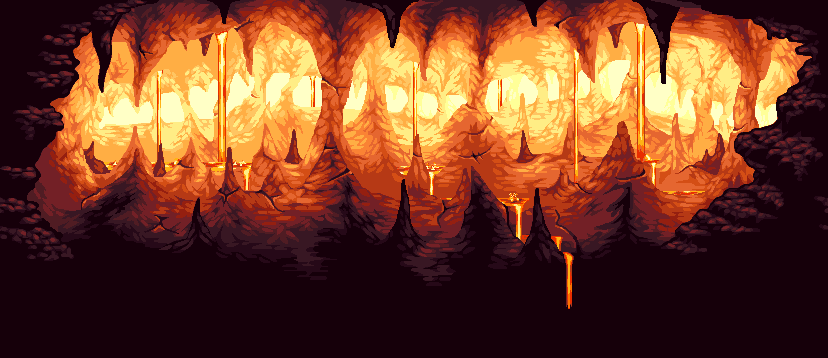
\includegraphics[width=0.9\textwidth]{photos/menu.png}
            \end{center}
        \subsection{Spielbare Charaktere und Inventar}
            \begin{center}
                \includegraphics[width=0.95\textwidth]{photos/charInv.png}
            \end{center}
         \subsection{Dungeon}
            \begin{center}
                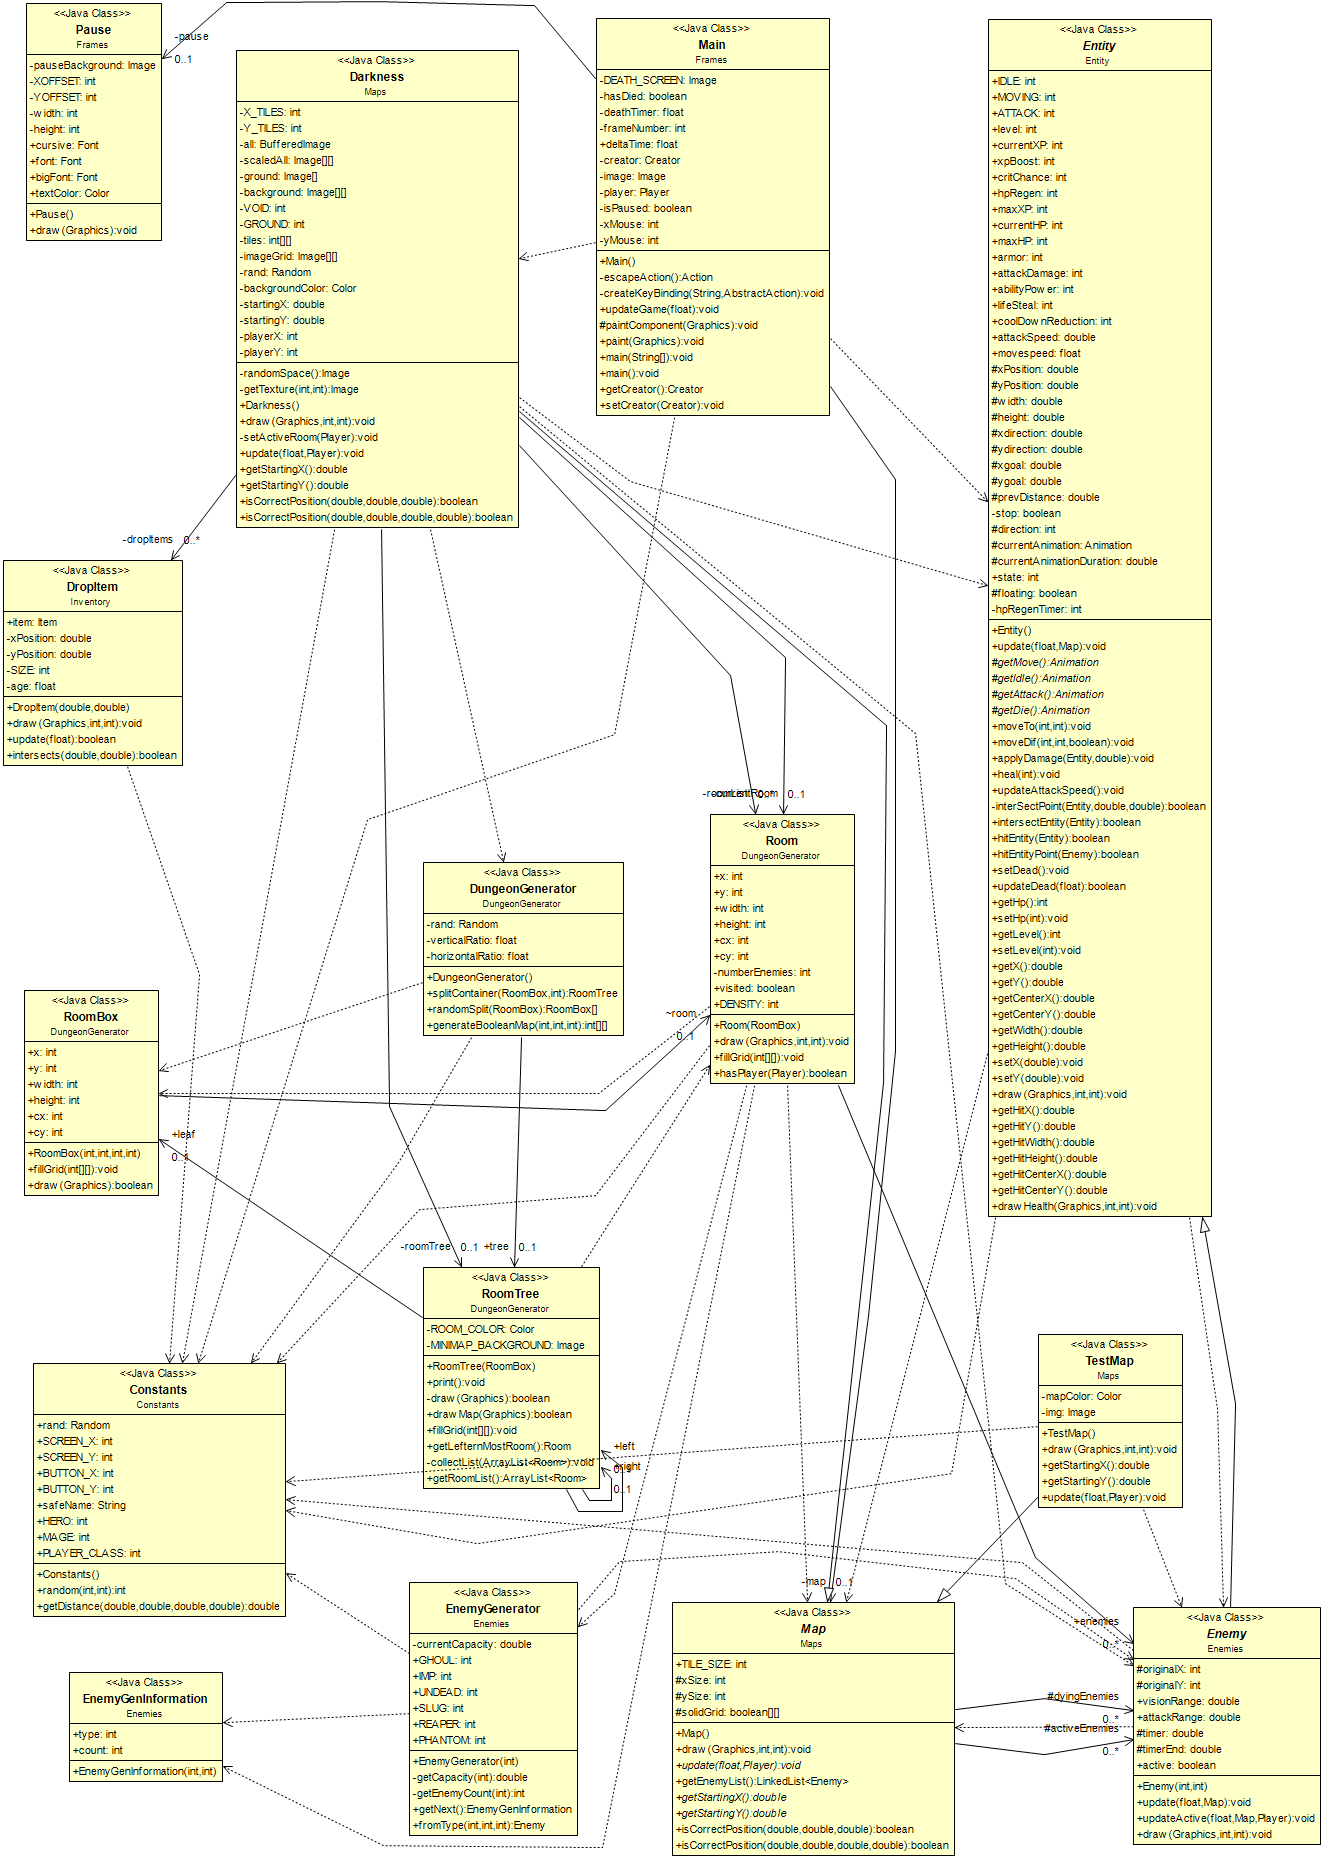
\includegraphics[width=0.95\textwidth]{photos/map.png}
            \end{center}
        \subsection{Kreaturen und Charaktere}
            \begin{center}
                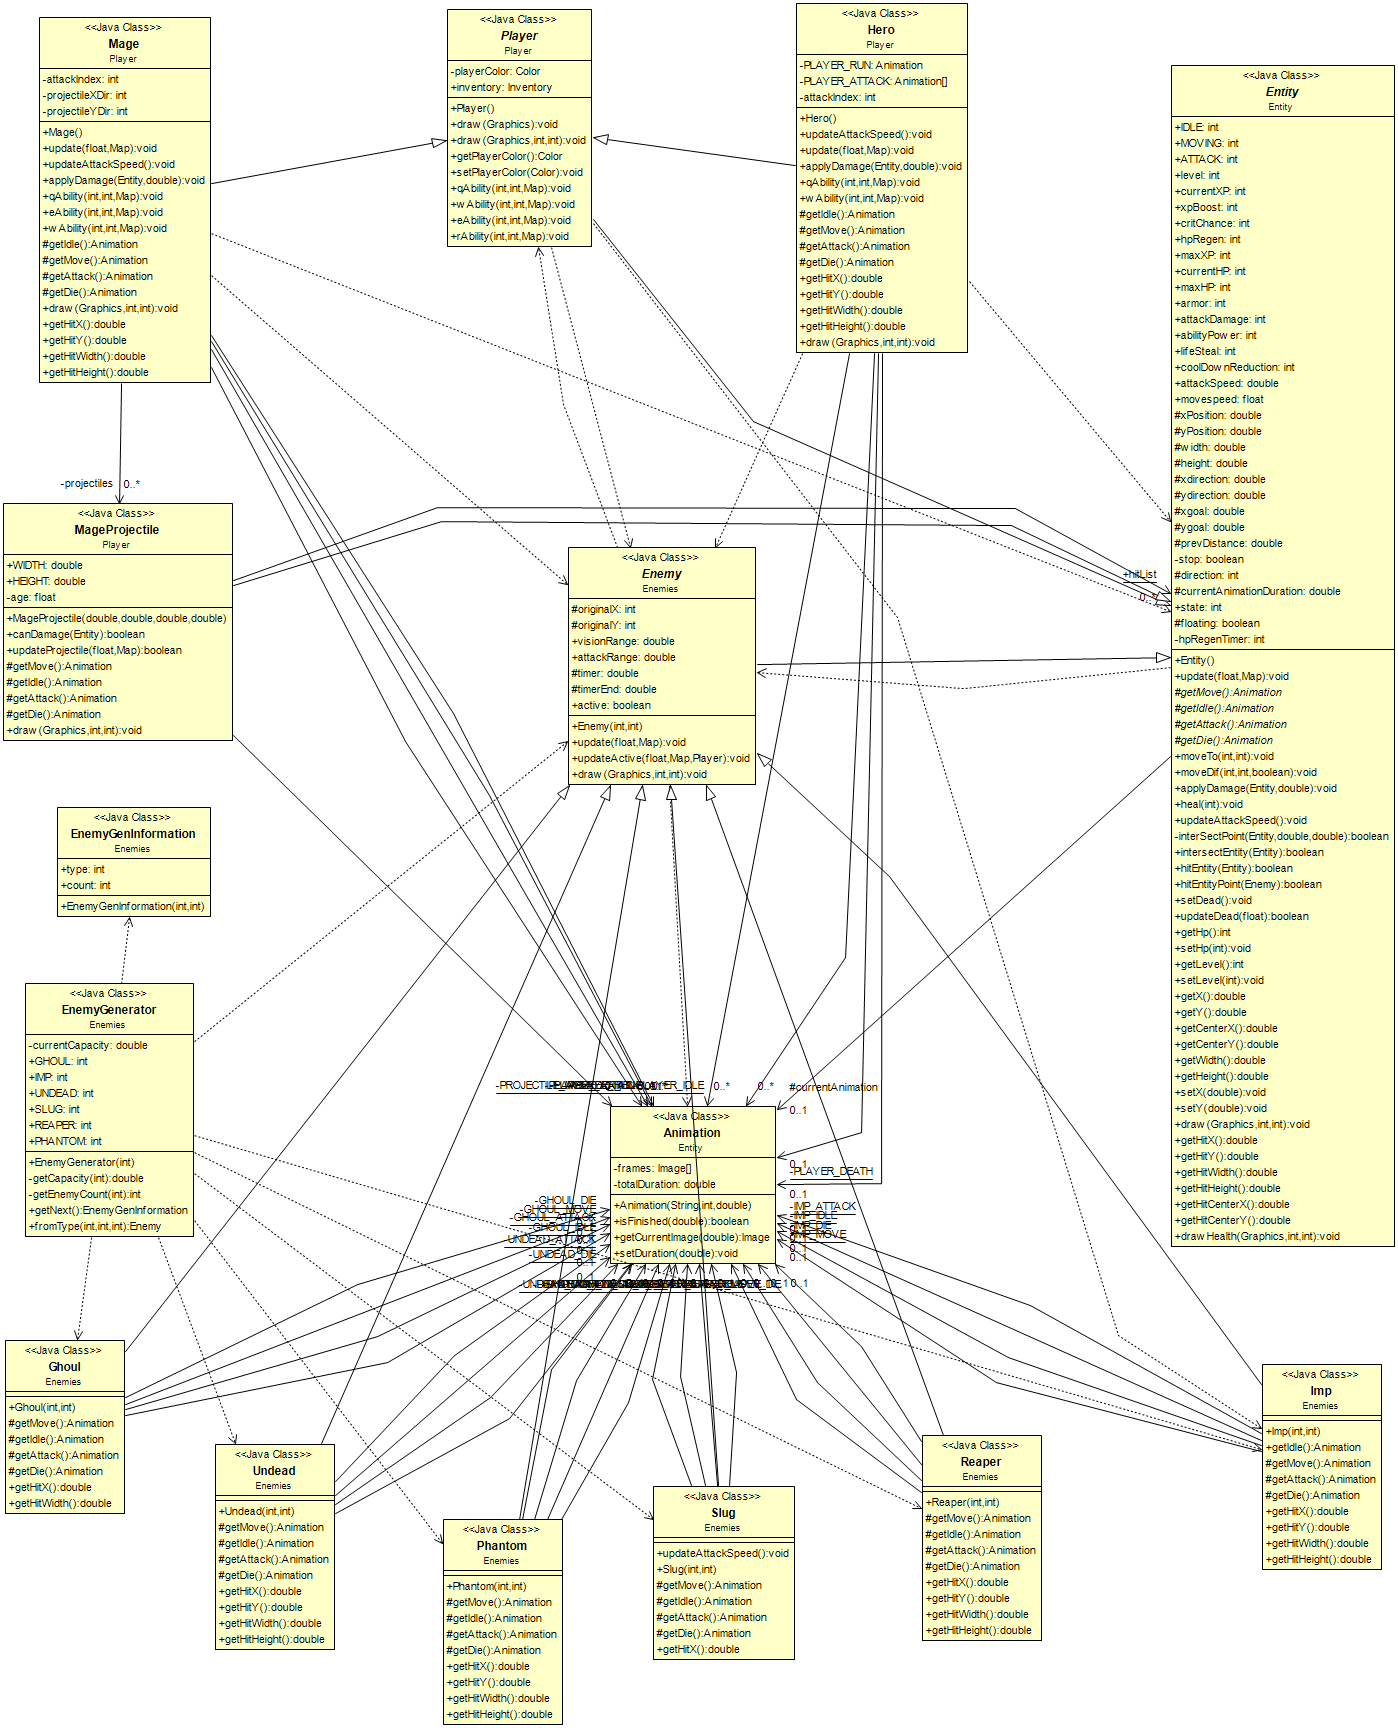
\includegraphics[width=0.95\textwidth]{photos/entity.png}
            \end{center}
        \subsection{Komplettes Klassendiagramm}
            \begin{center}
                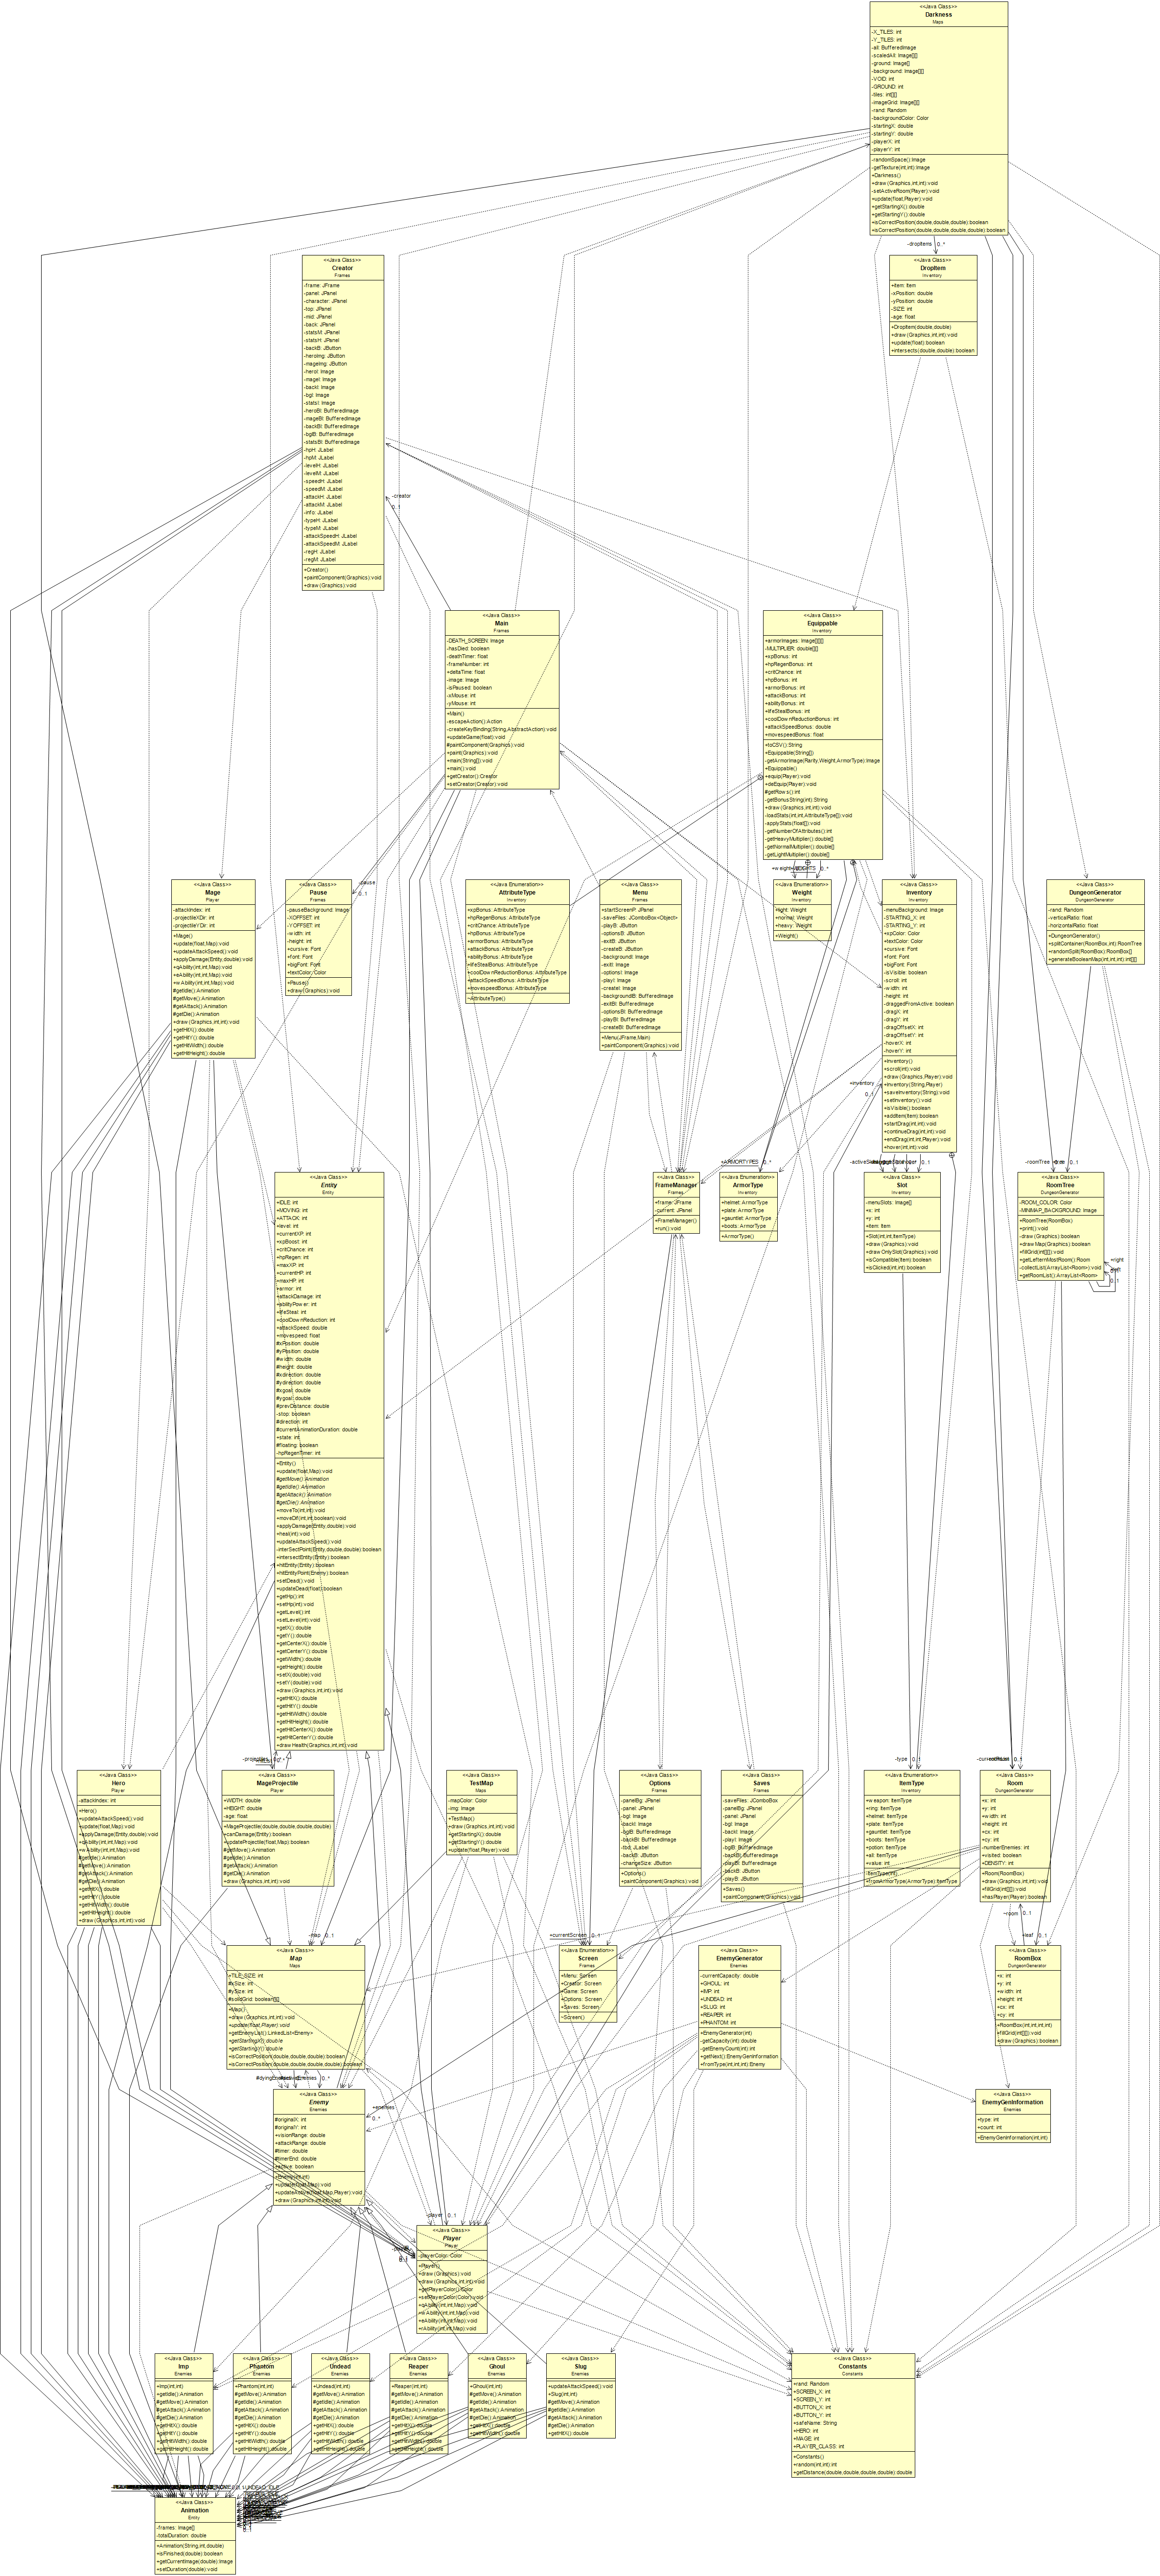
\includegraphics[width=0.65\textwidth]{photos/complete.png}
            \end{center}
            
\newpage
    \section{Dokumentation}
        \myuline{23.09.2019:} \\
            Tobias hat eine Vorlage für ein Eclipse-Projekt erstellt, die als Grundlage für das Softwareprojekt dient.
            Diese kann über den \glqq git clone\grqq{}-Befehl heruntergeladen werden und funktioniert über Eclipse.
            Außerdem enthält die Vorlage die Grafikbefehle, die als Grundlage für die grafische Oberfläche dienen sollen.\\
            
        \myuline{24.09.2019:} \\
           Jasper hat das Lastenheft in LaTeX erstellt. \\
         
        \myuline{24./25.09.2019:} \\
            Tobias hat eine \glqq Entity\grqq{}-Klasse erstellt.
            Diese soll die Oberklasse aller \glqq lebenden\grqq{} Spielelemente sein.
            Sie enthält funktionsvorlagen für das Aktualisieren sowie für das Zeichnen der Charaktere.
            Außerdem implementiert er die Funktion, dass sich Entities auf einen bestimmten Punkt bewegen können.
            Dies testete er durch die Steuerung eines Spielercharakters mit der Maus sowie eines Gegners, dem zufällige Positionen zugewiesen werden.\\
            Außerdem erstellte Tobias die abstrakte Klasse \glqq Map\grqq{}.
            Sie ist die Oberklasse für verschiedene Karten, die das Spiel haben soll.
            Die erste implementierte Karte ist die \glqq TestMap\grqq{}, welche verschiedene Spielmechaniken, wie die oben genannte, testet.\\
        
        \myuline{25.09.2019:} \\
           Jasper hat das Pflichtenheft in LaTeX erstellt.\\ 
           
        \myuline{25.09.2019:} \\
            Tobias und Yannick haben den Fensterwechsel zwischen Menü und Spiel implementiert.\\

        \myuline{26.09.2019:} \\
            Yannick hat diverse Ideen recherchiert, kam aber zu keiner guten Lösung\\

        \myuline{29.09.2019:} \\
            Tobias hat die Kamera auf den Spieler zentriert, sodass er sich bloß auf das Bewegen und nicht die Kamerasteuerung konzentrieren muss.
            Außerdem entwickelte er mehrere Fähigkeiten, die über die "q"-, "w"-, "e"- und "r"-Tasten ausgelöst werden  können.
            Diese sind in der Player-Klasse definiert und sollen in jeder Unterklasse unterschiedlich implementiert  werden, je nachdem, welche Klasse der Spieler ausgewählt hat.\\
            Zuletzt hat er die erste Map des fertigen Spiels begonnen.
            Diese wird durch einen zweidimensionales boolean-Gitter generiert.
            Die boolean-Werte enthalten Informationen darüber, ob ein Ort in der Map begehbar ist.
            Anhand diesem Gitter werden nun die nötigen Texturen geladen, sodass die Karte dynamischer wirkt, indem es z.B. Ecken und Vorsprünge gibt.
            Zuletzt hat er ein simples System zur Kollisions-Berechnung erstellt, sodass sich \glqq Entities\grqq{}, wie der Spieler, nur in eine Richtung bewegen können, wenn diese auch begehbar ist.\\

        \myuline{30.09.2019:} \\
             Tobias hat ein System für die Verwendung für Animationen, die sich aus mehereren einzelnen Frames zusammensetzten, erstellt.
             Hiermit können diese dynamisch und simpel geladen werden.
             Er hat Beispielanimationen für den Spielercharakter in Form von Renn-, Warten- und Kampfanimationen hinzugefügt.\\
             Anschließend hat er die Karten-Generation verbessert.
             Nun wird das boolean-Gitter über BSP-Bäume,die Räume zufälliger Größe (jedoch mit bestimmten Einschränkungen) generieren, erstellt.
             Außerdem hat er den Hintergrund von dem Vordergrund getrennt, sodass sich der Hintergrund langsamer als der Vordergrund bewegt und ein räumlicher Effekt entsteht.\\
        
        \myuline{01.10.2019:} \\
            Tobias hat ein System erstellt, welches den erstellten Räumen eine Liste von Gegnern zuweist und generiert.
            Hierfür kann man die relative Häufigkeit einer Gruppe eines bestimmten Gegnertyps sowie die Größer dieser Gruppe festlegen.\\
            Außerdem hat er sechs verschieden Gegner hinzugefügt, die eine Lauf- und Warteanimation besitzen.
            Das Kampfsystem ist jedoch noch nicht implementiert.\\
        
        \myuline{09.10.2019:} \\
            Jasper hat die (noch primitive) Charaktererstellung in das Hauptmenu implementiert. Des weiteren hat der das Menü und die Untermenüs um funktionierende zurück Buttons ergänzt. Es lässt sich auch nun das Spiel über die Charaktererstellung starten.\\
           
        \myuline{10.10.2019:} \\
            Jasper und Josh haben sich gemeinsam an Git und Eclipse gewöhnt, sodass sie nun weniger Angst davor haben. Dabei haben Sie den Charakterauswahlbildschirm um ein paar Eigenschaften des Spielers ergänzt, auch wenn diese noch auf keine Werte verweisen. Des weiteren haben Josh und Jasper an Key-Bindern herumexperimentiert, mit dem Ziel per Dinge wie das Pausenmenü zu steuern.\\
           
        \myuline{11.10.2019:} \\
            Tobias hat einen Inventarbildschirm erstellt.
            Dieser zeigt sowohl die Werte des Spielecharakters (Leben, Rüstung etc...) als auch die getragenen Gegenstände an.
            Man kann verschiedene Gegenstände ausrüsten, die die Stats des Spielers dann verbessern.
            Außerdem wurde ein System zur Erstellung von Items erstellt, dass Items zufällige Werte zuweist.\\

            \myuline{12.10.2019:} \\
            Tobias hat das Itemsystem verbessert.
            Die erstellten Items haben nun Werte, die neben zufälligen Faktoren auch von der Art und Seltenheit des Gegenstandes abhängig sind.\\

        \myuline{13.10.2019:} \\
           Jasper hat die Klasse Optionen erstellt. Dann hat Jasper angefangen sich über Hintergrundbilder und schönere Buttons zu imforieren und daran zunächst lange erfloglos, herumexperimentiert.\\
           
        \myuline{14.10.2019:} \\
            Jasper hat einen Durchbruch bei den Hintergrundbildern erreicht. Dank dessen haben nun die verschiedenen Menüs wunderschöne Hintergrundbilder.\\
            
        \myuline{16.10.2019:} \\
           Jasper hat die Klasse Magier erstellt. Diese ist der zweite Spielbare Charakter, welcher auch schon in der Charaktererstellung zu sehen ist. Das Übergeben des Charakters für den sich der Spieler entschieden hat, muss jedoch noch implementiert werden.\\
           
        \myuline{18.10.2019:} \\
            Tobias hat das Nahkampfsystem der \glqq Entities\grqq{}-Klasse fertiggestellt.
            Hierfür hat er die Hitboxen der einzelnen Klassen überarbeitet.
            Zuletzt hat er gestorbenen Gegnern eine Todesanimation hinzugefügt.\\

        \myuline{19.10.2019:} \\
            Jasper hat verschiedene Varianten versucht, wie man den ausgewählten Charakter an das Spiel übergeben kann. Auch wenn er heute daran gescheitert ist, gibt er nicht auf, des weiteren gilt ja bekanntlich: Der Weg ist das Ziel!\\
           
        \myuline{19.10.2019:} \\
            Joshua hat am Pausenmenu weitergearbeitet und es fast fertig gestellt. \\
           
        \myuline{19.10.2019:} \\
            Tobias hat die Fernkampffähigkeit der Magier \glqq Mage\grqq{}-Klasse implementiert.
            Dieser schießt ein Geschoss, welches Gegner durchdringt und in alle Richtungen geschossen werden kann.\\

        \myuline{19.10.2019:} \\
            Yannick hat das Menü verbessert, kleine Codfixes vorgenommen, nicht benutzte Bilder gelöscht und erste Recherchen und Versuche zu den HPBars vorgenommen und getestet (Erfolglos).\\

        \myuline{20.10.2019:} \\
            Joshua hat das Pausenmenu bis auf kleinere Fehler fertiggestellt und funktionstüchtig gemacht.\\
           
        \myuline{20.10.2019:} \\
            Jasper hat die Buttons in dem Menü vereinheitlicht, damit diese überall gleich groß und designtechnisch konsistent sind. Jasper hat es außerdem mit ein wenig Hilfe von Tobias geschafft, die Charactererstellung funktionstechnisch fertig zu machen. Der nächste Punkt auf Jasper Tages- bzw. Sonntagabendordung war das Verschönern von der Charaktererstellung zu dem was aktuell zu sehen ist. Des weiteren hat Jasper die Eigenschaften der Charaktere vervollständigt und diese verweisen nun auf die tatsächlichen Werter der jeweiligen Klasse. Danach folgten noch das Zusammenführen der Entwicklungszweige auf den Master zusammen mit Yannick und Tobias.\\
           
        \myuline{20.10.2019:} \\
            Tobias hat die Minimap verschönert.
            Außerdem hat er die Lebensanzeige des Spielers hinzugefügt.\\
            Gegner haben nun eine Chance, nach ihrem Tod ein Item fallen zu lassen. Dieses kann vom Spieler eingesammelt werden.
            Außerdem hat er die Angriffsgeschwindigkeit und Lebensregenerationsstats implementiert.
            Außerdem hat er das Itemsystem verfeindert, sodasss man mehr Kontrolle über den Wertebereich der einzelnen Stats hat.\\
            Zuletzt hat grundlegende Spielstände implementiert.
            Diese Speichern jedoch zum aktuellen Zeitpunkt nur das Inventar des Spielers, nicht aber die Klasse oder die Position auf der Karte.\\

        \myuline{21.10.2019:} \\
            Tobias hat einen Bildschirm erstellt, der erscheint, wenn der Spieler stirbt.
            Es wird nun in diesem Fall verhindert, dass der Spieler sich weiter bewegt.
            Es wird eines Todesanimation abgespielt und man wird nach drei Sekunden in das Hauptmenü weitergeleitet.\\
            Außerdem hat er ein Problem mit den Hitboxen behoben, den Stats der Gegner zufällige Werte zugewiesen sowie einen Lebensbalken für Gegner implementiert.\\
            Zuletzt hat er verhindert, dass Gegner auf der Insel erscheinen, in der das Spiel startet, sodass sich der Benutzer besser auf den Kampf vorbereiten kann.\\

        \myuline{18.10.2019:} \\
            Yannick hat die Menüs umgeordnet, das Spiel auf Buggs getestet, einige gefunden, beschlossen, dass es Features sind und Versucht die HPBar zu fixen und zu ändern.\\
            
\end{document}
%-------------------
%Hier endet der Text deiner Hausarbeit
%-------------------